\section{Fundamentals of Evolutionary Algorithms}

\subsection*{Random local search and the (1+1) evolutionary algorithm}
In this section, we will introduce the basic concepts of evolutionary algorithms, starting with \italic{random local search} and the \italic{(1+1) evolutionary algorithm}. Those are two fundamental algorithms that are used as building blocks for more complex evolutionary algorithms and offer deep insights into the challenges in the field. \\ 
Figure \ref{fig:EAvsNature} sketches the fundamental ideas of evolutionary algorithms and contrasts it to its inspiration: evolution in nature.  \\
\begin{figure}[H]
  \centering
  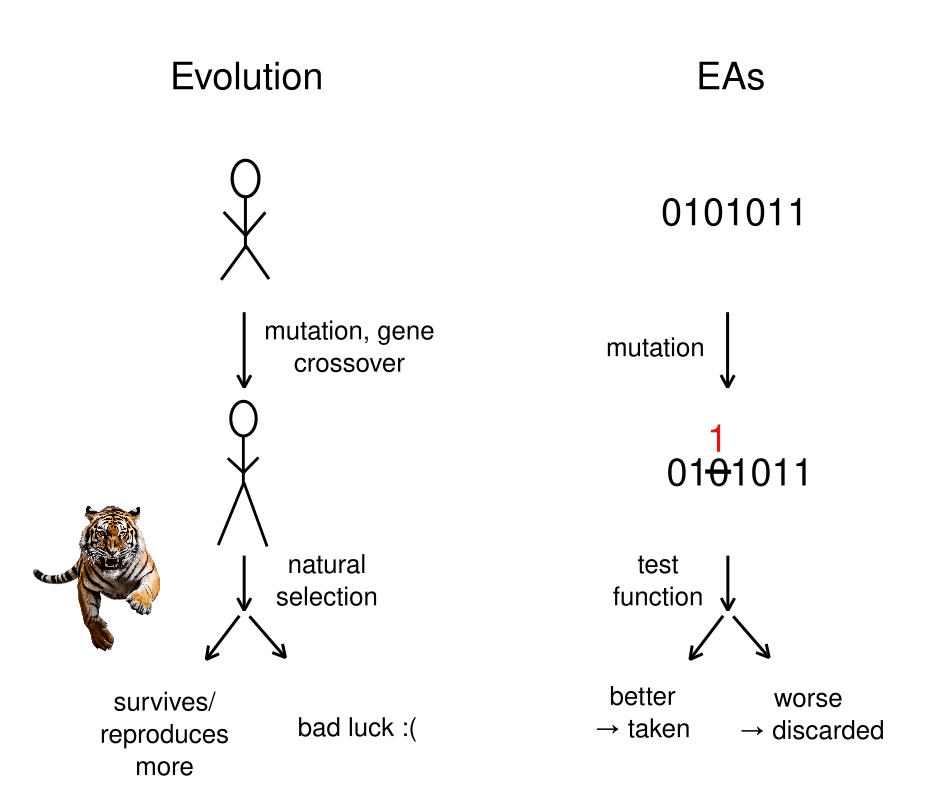
\includegraphics[width=0.51\textwidth]{images/evolution_analogy.png}
  \label{fig:EAvsNature}
\end{figure}
Darwin's theory of natural selection considers the long-term adaption of a species to its environment. It suggests that individuals with advantageous traits are more likely to survive and reproduce, thereby passing those traits to future generations.\\ 
Evolutionary algorithms fundamentally work in the same way. Only, instead of animal or plant species bitstrings or other representations of potential solutions are evolved. Here, we will focus on binary strings, but the principles can be transferred to other representations and real-life problems as well. \\
For an evolutionary algorithm you always need some function that takes a bitstring, in this context often called individual, and changes any number of its bit. This step is called mutation and often is non-deterministic. In a next step the EA determines if the new individual is better than the old one. For this, a so called fitness or test function is used. This function takes an individual and returns a value that represents how well the individual adapted to the given function. The goal of the EA is to maximize this value. Finding a suited fitness function for a real-life problem can be very challenging and is crucial for the success of an evolutionary algorithm. \\
The following pseudocode shows how random local search and (1+1) EA work.\\[2ex]
\noindent
\begin{minipage}{0.48\textwidth}
\textbf{Random local search (RLS)}
\begin{algorithmic}
\State Sample $x \in \{0, 1\}^n$ uniformly at random
\For{$i = 1$ to $\infty$}
  \State $y \gets flipOne(x)$
  \If{$f(y) \geq f(x)$} $x \gets y$
\EndFor
\end{algorithmic}
\end{minipage}
\hfill
\begin{minipage}{0.48\textwidth}
\textbf{(1 + 1) Evolutionary algorithm (EA)}
\begin{algorithmic}
\State Sample $x \in \{0, 1\}^n$ uniformly at random
\For{$i = 1$ to $\infty$}
  \State $y \gets mutate(x)$
  \If{$f(y) \geq f(x)$} $x \gets y$
\EndFor
\end{algorithmic}
\end{minipage}
The main difference between the two algorithms is the mutation function. \textbf{Random local search} mutates indivuals by randomly choosing one of the n bits and inverting it. \textbf{(1 + 1) EA} on the other hand uses a mutation function that flips each bit with a probability of $\frac{1}{n}$. Consequently, in each iteration of the (1 + 1) EA, between $0$ and $n$ bits of the indivual can be flipped, while \textbf{RLS} always flips exactly one. \\

\subsection{Test Functions}
As already mentioned, the chosen fitness function is of utmost importance for the success of an evolutionary algorithm. While fitness functions of real-life problems can be very complex and hard to define, we will focus on simple test functions in these analyses. \\
As most of the discussed functions are not very complex only a brief definition, an explanation and a short example will be given.\\
\subsubsection{OneMax}
The fitness function \textit{OneMax} assigns to each bit string italic{x} the number of one-bits in x \cite{oneMax}. It can be defined as follows:
$$ \text{OneMax}(x) = \sum_{i=1}^{n} x_i $$
where $x_i$ is the i-th bit of x.\\
Some things to note about this fitness function is, that \textit{oneMax} is has some attributes, that simplify evolutionary algorithms   significantly when run with these. For example, this function possesses exactly one optimum that being the string consisting only of ones. This optimum being the only one consequent also is the global optimum.   TODO: INSERT STUFF HERE LIKE MONOTICALLY INCREASING; HAS EXACTLY ONE OPTIMUM WHICH IS THE GLOBAL OPTIMUM \\ 
An extension of \textit{oneMax} are \textit{linearFunctions}. These test functions assign every bit $x_i$ a real weight $w_i$. The definition of \textit{linearFunctions} is as follows:
$$ \text{linearFunctions}(x) = \sum_{i=1}^{n} w_i \cdot x_i $$
where $x_i$ is the i-th bit of x and $w_i$ is the weight of the i-th bit.\\

\subsubsection{LeadingOnes}
\textit{LeadingOnes} is a function that assigns to each bit string \textit{x} the length of the longest prefix of \textit{x} that consists of one-bits \cite{leadingOnes}. It can be defined as follows:
$$ \text{LeadingOnes}(x) = \sum_{i = 1}^{n} \prod_{j = 0}^{i}x_i $$
where $x_i$ is the i-th bit of x.\\

\subsubsection{Needle}
Evolutions algorithms often rely on the fitness function to incrementally lead to the optimal or at least close-to optimal solution by iteratively improving the current solution. The \textit{needle} function is a test function that is designed to make this very difficult. Only the bit string consisting only of ones has a fitness bigger than zero while any other bit string has the fitness zero. This means, an evolutionary algorithm has no way of approaching the optimal solution, but instead has to encounter it randomly. It is looking for the figurative needle in a haystack. It is defined as follows:
$$ \text{needle}(x) = \begin{cases} n & \text{if } x = 1^n \\ 0 & \text{otherwise} \end{cases} $$
where $x = 1^n$ is the bitstring of length n that consists only of ones.\\
